\documentclass{article}
\usepackage{graphicx}
\begin{document}
\section{Working Within the Group}
As a part of working within the group, we have had various different ways of working together. 
At the beginning when we started writing our problem analysis, each person got a section they had to investigate and write about. 
When the problem analysis was written, we moved on to the development stage. 
In the development state we did the same as before, but this time split the group up into smaller groups to divide the workload. 
Each group got the task of constructing and finishing the various parts of our programme and documentation thereof. 
With regards to correcting our report, we read the whole report together and came with our individual corrections and helped each other complete the task that way.

We have also had to try and plan our time effectively. 
This was done by creating a schedule that covered the whole semester. 
However, along the way, we created some smaller deadlines, to help keep us aware that we had deadlines to reach, and creating them and discussing them througout the project, helped with keeping them fresh in our minds.

We have not had any extraneous group activities. 
We do not feel as though this has been detrimental to our process. 

\section{Working with the Supervisor}
At the first supervisor meeting we came to the agreement that material should be sent 24 hours in advance, unless otherwise agreed upon. 
We had also agreed on providing the supervisor with an agenda for our meetings, so that there was no confusion on what was to be focused on at the meetings. 
Our original idea was to write create a formal agenda, but it ended up with being more of a discussion, where we wrote to Kurt what we had done and what we wanted to discuss at the meeting. 
We feel that this has gone well, as we feel that at every meeting we held with Kurt, we received a lot of information as to how we can improve our work and how we can further our project.

\section{Project Management}
\subsection{Group Contract}
At the beginning of the project we created a group contract. 
Everyone in the group was in agreement with the various conditions the contract set at the time of creation. 
The agreements within this contract, will be described in a little more detail in the following sections.

\subsection{Project Leader}
For this project we decided to have a project leader, to take control of the group for a week at time. 
This was a role that everyone was supposed to try at some point during the course of the project. 
The project leader role consisted of making sure that the group held concentration and did not get too sidetracked, coordinate meetings and keep in contact with our supervisor. 
Another task the project leader had, was to update our Trello board.
We realised after the first time someone had tried being group leader, that one week was simply not enough for them to get accustomed to the role of project leader.
Not every group member had the same enthusiasm for the role. 
Some were better at taking command than others especially in concern to taking control of the group.
The task of updating our Trello board, did not go quite as planned. 
It ended up with it being the person who wrote a summary of any meetings that updated the board.

\subsection{Attendance}
Througout this semester, we have taken attendance. 
Every time the group had a meeting or a lecture, attendance was taken. 
This was done to ensure that we had concrete details on when a person was present or not. 
If attendance came under 80\%, we had agreed that the person had to talk to the project leader and find out why their attendance had been so poor. 
If attendance came under 65\%, the person in question had to be evicted from the group. 
We thought it necessary to have details of attendance, so that if it did become a problem, we could show the person solid evidence of their absence. 
The reason for taking absence was based on past experiences of half the members of the group. 
Taking attendance could also lead to some form of motivation for people showing up when meetings are held.
On figure \ref{fig:GraphImage}, we have the general oversight of the group's attendance. We can also see when a specific group member has been absent as seen on figure \ref{fig:soerenfravaer}.
An issue that we came upon when starting this project, was taking attendance at the start of the semester. 
As if a person was absent just two days into the project, their absence would be incredibly high. 
So something that should have been discussed further, was when we started enforcing the attendance rule. 
This semester, attendance has not been a large issue. 
It is unknown whether it was our attendance taking that did this, or whether it was just the different group members that were more motivated.
We have discussed that even if a group member came down to 65\% it was necessary to discuss further and see why absence had become so poor instead of drawing the line at 65\%, with no exceptions.

\begin{figure}
	\centering
	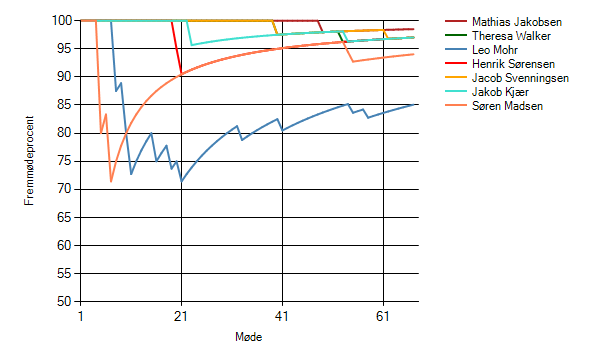
\includegraphics[width=1\textwidth]{figures/GraphImage.png}
	\caption{An oversight of the group's absence}
	\label{fig:GraphImage}
\end{figure}

\begin{figure}
	\centering
	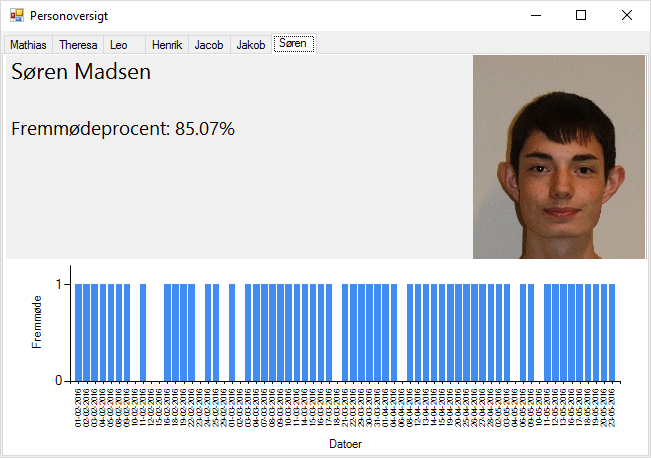
\includegraphics[width=1\textwidth]{figures/soerenfravaer.png}
	\caption{A specific group member's attendance sheet}
	\label{fig:soerenfravaer}
\end{figure}

\section{Learning Process}
In this project, we have used various tools to communicate, share documents and plan upcoming meetings with each other. 
We discussed that we would not use Facebook to communicate with each other to keep forms of communication professional. Another issue with using Facebook, is that not every group member had an account.
Instead, we have used Slack, an alternative method of communicating with each other. 
This programme was only used for talking to other group members and sharing relevant information.
We also used a website, Trello, that allowed us to write and see what our report was missing and when we had meetings. 
Towards the end of this project Trello was almost exclusively used as a way of documenting our meetings and saving the summaries of these meetings, instead of writing parts of the report that are missing. 
This was, instead, done by discussing amongst ourselves at our weekly meetings.


\section{Cluster Group}
This project has had a different element to it. We have had to work with two other groups and try and get these groups to work together.
\subsection*{Concerns}
There have been a number of cluster meetings with the groups from Mathematics (MAT) and Internet Technologies and Computer Systems (ITC), and us, Computer Science (DAT), as well as with each group's project supervisors.
In the beginning there was a bit of uncertainty in our group about how the entire process would work, since each group in the cluster had a different curriculum and a different set of requirements to be fulfilled.
Furthermore, we were concerned about the fact that each group had to figure out a part of the whole solution based on the work of others.
Essentially, it sounded like MAT would develop an algorithm as a base for us (the Computer Science group) to use.
DAT would then use this algorithm and develop a class library for the ITC group to use.
ITC would finally use the algorithm and the library in their project.
This would require a lot of time and be largely inefficient, since one step of the process had to be completed before another one could begin, and we only had about four months for the project in total.
It would also mean that ITC would be dependant on DAT, while DAT would be dependant on MAT for their respective projects, and that would not be feasible.
In a similar vein, the point of the cluster group was that each group could benefit from the work of others.
But how could our group benefit from the work of ITC if they were dependant on us? And would MAT gain any benefit from the cluster group at all?

We brought these concerns to the table at the first cluster meeting with each group's advisor and Hans Hüttel, who made the project proposal.

\subsection*{Trying to work together}
There was no real progress in the cluster collaboration during the first weeks, which was expected, as we were all finding out which direction we wanted to take.
Everyone was busy learning about steganography and how to use it.
Our group made a fairly trivial programme to embed data into other data using least significant bits, but we could not spend the entire project on that. However, this programme was not completely useless with regards to ITC, as ITC could use it, and it was decided that DAT would deliver either that or whichever better programme that was developed later.

Olav Geil, MAT's advisor, held a lecture on an article about a graph-theoretic approach to steganography.
This proved to be valuable to both us and MAT, as both groups would later decide to use this approach in some form.
DAT and MAT somewhat connected over this, thinking this could be the key to the lacking collaboration.
We were encouraged by the supervisors to collaborate, perhaps letting MAT develop and giving us an efficient algorithm using this approach, while DAT developed a slightly less efficient algorithm for testing purposes until MAT was done with their investigations.
When voicing concern about how MAT would benefit from this, we were told that it could possibly be exciting for them to see their algorithm in action.

To solidify the demise of the cluster project, we realised at a cluster meeting - roughly a month before the final deadline - that DAT and MAT had chosen different paths.
MAT had dedicated their time to make the algorithm presented by Olav Geil as precise as possible, sacrificing efficiency, while DAT were looking for an efficient algorithm where extreme precision had less of a priority.
This meant that MAT and DAT would be of no use to each other, and it was decided that it was the end of the collaboration between DAT and MAT.
ITC will still get a complete steganographic solution to use as a library with select methods exposed, since they will have no use of the entire codebase in their project.

Syntese
 - Vi vil starte med at
 - Vi vil fortsætte med at
 - Vi vil holde op med at
\end{document}